\documentclass[11pt]{article}
\usepackage[review]{acl}
\usepackage{times,latexsym}
\usepackage[T1]{fontenc}
\usepackage[utf8]{inputenc}
\usepackage{microtype,inconsolata,booktabs,amsmath,amssymb,graphicx}
\title{What Does a Persona Add? Separating Instruction Effects from Predictive Mixture Gains}
\author{Anonymous authors}
% lineno 5.7 compatibility: switch placement only; no layout changes.
\makeatletter
\AtBeginDocument{\renewcommand\makeLineNumber{\logtheLineNumber\getLineNumber\if@firstcolumn\makeLineNumberLeft\else\makeLineNumberRight\fi}}
\makeatother
\begin{document}
\maketitle
\begin{abstract}
Persona-conditioned language models can predict a person's responses, but this does not establish that persona wording adds value beyond the same observed history. We distinguish three comparisons: matching the person, changing the instruction, and augmenting a statistical predictor. Across two model families and two survey instruments, these comparisons yield different conclusions. In a historical 84-template experiment, the planned optimizer comparison did not establish superiority. On a further same-inventory panel, a frozen Granite mixture beat neutral mixtures at a small decoder-fitting budget, but statistical predictors led at every examined budget from 320 people onward. On 658 held-out respondents from a public external survey, Granite mixtures using neutral or an unadapted transferred instruction modestly improved over a full-data statistical control under the internally frozen analysis; Qwen intervals included zero. A statistical-only stimulus-prior mixture improves over that control by a larger point estimate. Yet the direct comparison of the CAL-selected Granite mixtures was near zero. Post-review statistical-only mixtures remove evidence of an LLM advantage: Granite superiority over stimulus-conditioned empirical shrinkage is not established; no equivalence margin was declared. Granite-versus-decoder intervals also include zero when calibration-weight selection is resampled. These results support evaluating instruction effects separately from mixture gains, with explicit supervision budgets, stimulus alignment and conditional uncertainty.
\end{abstract}

\section{Introduction}
A plausible simulated respondent need not predict the unseen responses of a particular human. Even a predictor that benefits from that person's profile need not benefit from an optimized persona instruction. This distinction matters when language-model simulations are proposed as substitutes for collecting human answers.

We ask a narrow question: what additional predictive value is obtained by changing a reusable persona instruction, relative to a neutral instruction and statistical use of the same observed history? Our evidence concerns probability forecasts of individual questionnaire answers and hypothetical choices, not human-like behavior or actual purchasing. We compare reusable templates that are instantiated from each person's observed history; no test-person target answers are supplied to the template.

Three comparisons are necessary. A matched-versus-wrong-person profile contrast measures the value of assigning the history to its owner. A persona-versus-neutral contrast holds that history fixed and tests an instruction-specific forecast package. A mixture-versus-decoder contrast asks whether language-model forecasts improve a specified statistical component. These are different estimands. We show how treating these comparisons as interchangeable produces conflicting conclusions; the person-matching contrast is available only on IPIP.

The contribution is an empirical evaluation procedure and its application across two instruments, not a new optimizer or the first comparison with regression. We combine exact-history and representation controls, explicit fitting-budget curves, stimulus-matched external forecasts, and direct comparisons of instruction-specific mixtures under the same CAL-selection rule. We preserve the planned null, model-dependent effects and post hoc status of subsequent analyses. The resulting evidence ladder changes the conclusion: fixed Granite mixtures improve a specified decoder, but neither an advantage over statistical-only pooling nor stability to calibration-sample variation is established. This distinguishes a conditional component gain from evidence that an LLM or a persona instruction is needed.

\section{Related work}
\citet{hu2024persona} already quantify persona effects and compare LLM predictions with supervised linear regression. We extend this line through budget-dependent comparator selection and the distinction between instruction-specific and mixture gains. Persona simulations based on interview or survey information~\citep{park2026selfreports}, and learned models of cognition~\citep{binz2025centaur}, address a broader range of human prediction. Our fixed-input comparison does not establish comparable behavioral or task generalization.

Population resemblance is another distinct target. Demographic conditioning can recover aggregate patterns~\citep{argyle2023samples}, yet similar means can coexist with distorted variation and associations~\citep{bisbee2024synthetic}; LLM survey biases can also differ from human biases~\citep{tjuatja2024biases}. We therefore evaluate paired individual proper loss. Twin-2K-500~\citep{toubia2025twin} supplies the external survey; its participants and randomized stimuli are existing resources, not our contribution. Our stimulus audit repairs our initial adapter's misuse of presentation slots.

The historical search comparison includes adapters inspired by EvoPrompt, PromptBreeder, OPRO, ProTeGi and GEPA~\citep{guo2024connecting,fernando2024promptbreeder,yang2024opro,pryzant2023protegi,agrawal2025gepa}. Those experiments motivate the evaluation question; their complete methods and negative comparisons remain in the self-contained Supplements S2 and S4.

\section{Evaluation design}
\subsection{Three distinct contrasts}
Let $x_i$ denote permitted history, $y_{ij}$ a withheld response and $P_g(x_i)$ the forecast from instruction $g$. Let $R(x_i)$ be a fitted statistical decoder, $g_0$ neutral wording and $\pi(i)$ a different person. With lower proper risk $\mathcal L$ better, we distinguish
\begin{align}
D_{\mathrm{match}}&=\mathcal L(P_g(x_i))-\mathcal L(P_g(x_{\pi(i)})),\\
D_{\mathrm{instruction}}&=\mathcal L(P_g(x_i))-\mathcal L(P_{g_0}(x_i)),\\
D_{\mathrm{mix}}&=\mathcal L(H_g(x_i))-\mathcal L(R(x_i)).
\end{align}
For fixed fitted pipelines, $\mathcal L(P)=\mathbb E_i[\sum_j a_j\ell_j(P_j(x_i),y_{ij})]$, estimated by the participant average. We set $a_j=1/60$ and $\ell_j=L$ on IPIP; on R2, $a_j=1/(2|F(j)|)$ and $\ell_j=L_j/c_j$, where $F(j)$ is the endpoint's family and $c_j$ its frozen CAL prior loss. Expectations concern people from the same task population, not new endpoints. These are distinct design questions, not three contrasts implemented in every dataset: R2 lacks the deranged-history test.

Here $H_g=(1-w_g)R+w_gP_g$ is linear probability pooling~\citep{gneiting2011combining}. Comparing $H_g$ with $H_{g_0}$ requires specifying whether $w_g=w_{g_0}$ or whether each weight is selected using the same calibration rule. For R2 component contrasts, $R=R_{\rm comp}$; for the original comparator contrasts, $R=R_{\rm ref}$, while $H_g$ always pools $R_{\rm comp}$. The latter instruction comparison tests deployable instruction-specific packages; it need not recover a prompt-only effect. Likewise, a negative $D_{\mathrm{match}}$ does not imply either other contrast is negative.

\subsection{IPIP history and statistical controls}
In IPIP-NEO-120~\citep{johnson2014ipip}, 60 observed items predict 60 disjoint target items. The renderer compresses the history into 30 facet and five trait categories. LLM arms share this renderer. Statistical controls receive either raw one-hot answers or the exact categorical profile; the latter tests whether access to uncompressed answers alone explains a gap.

For five ordered responses we use normalized ranked probability score (RPS),
\begin{equation}
L(p,y)=\tfrac14\sum_{k=1}^4\left(\sum_{h=1}^kp(h)-\mathbf1\{y\le k\}\right)^2.
\end{equation}
We average target losses within person before averaging people. Proper scoring rules reward calibrated probability forecasts~\citep{gneiting2007proper}. Reverse-keyed items are mapped to the corpus's recoded scale. Readout uses returned digit-token probabilities with a documented uniform fallback for zero digit mass. Calibration anchors predicted CDFs to training priors, fits shrinkage on a distinct calibration split and projects onto valid CDFs.

The historical readouts are Qwen3.6-35B-A3B and Granite-4.2-30B with a Qwen3.8-27B mutator. Eleven search identities and three objective variants yield 84 final cells across two models and three seeds. Original train/search/select/calibrate/evaluate panels contain 8,000/80/120/120/600 people. Templates and decoders are frozen before final evaluation. Complete source settings and grids are in Supplements S2 and S4.

We use E3 for the third IPIP evaluation panel, B1 for its budget reanalysis, R2 for the corrected external protocol, and T0 for an unadapted transferred instruction component. CAL denotes calibration data.

The E3 follow-up freezes historical Granite persona--ridge recipes and neutral mixtures on a third, disjoint 600-person same-corpus panel. At this stage the ridge fitting budget is 80, but the hybrid also uses historical search, prior, selection and calibration labels. The subsequent B1 analysis reuses E3 outcomes and selects prior, ridge or nonlinear statistical predictors by within-training three-fold cross-validation at 80, 160, 320, 1,000, 8,000 and 8,320 fitting people. Raw and categorical features receive separate selection. These curves compare specified pipelines, not equal total supervision or computation.

\subsection{External stimulus-matched forecasts}
Twin-2K-500 supplies 2,058 people, split into FIT/DEV/CAL/TEST of 1,000/200/200/658. Forty endpoints are hypothetical purchase choices, eight are ordinal benefit/risk ratings and one is binary. Models and controls receive the same 229 permitted Wave-1--3 history columns; target and semantically overlapping blocks are excluded. The transferred T0 is an instruction component, not the full IPIP genotype. Its inherited text refers to intensity prefixes and facets, although R2 supplies numerical answer history without those prefixes. This deliberately unadapted component transfer cannot test the value of a domain-adapted persona; exact text is in Supplement S1.

Product identifiers in the source catalog index presentation slots rather than a constant product at a constant price. Our initial adapter treated them as constant. The corrected R2 crosswalk binds each forecast to the individual's actual product, price and ordered options. Among 82,320 offers, only 220 exactly match the catalog example. This is a correction to our adapter, not a discovery about flaws in the original study. R2 was frozen after the earlier history-only CAL diagnostic but before its own fitting and model forecasts.

The statistical component decoder1200 uses FIT and DEV, with cross-validated candidate selection inside those 1,200 people. Full1400 repeats candidate-family, feature-source and hyperparameter selection and fitting on FIT+DEV+CAL. It is not merely a refit of the selected decoder1200 specification. We distinguish the component $R_{\rm comp}$ (decoder1200) from the equal-label-budget comparator $R_{\rm ref}$ (Full1400). Each LLM instruction is evaluated standalone, mixed at weight 0.5, and mixed with a weight selected on CAL separately for each endpoint using a common frozen grid, objective and tie rule. All TEST predictions are evaluated only after weights are frozen.

Binary/nominal targets use log loss; ordinal targets use normalized RPS. Each endpoint's loss is divided by its frozen CAL prior loss. The original aggregate gives equal weight to the economic and heuristic families, then equal weight within family. Thus it is dimensionless and not a percentage reduction against Full1400. Raw losses of different kinds are not pooled into an unnormalized risk.

\subsection{Uncertainty and evidence chronology}
Our inferential unit is the participant. All paired contrasts condition on fitted models, selected templates and forecasts. Historical crossed bootstrap intervals also resample three observed search seeds; they are descriptive sensitivity to those runs, not reliable uncertainty over future searches. Historical respondent sign-flip tests condition on these runs and require the relevant symmetry/exchangeability assumptions; they are not obtained by inverting the crossed interval procedure.

The original search family contains 110 comparisons. E3 has four declared comparisons and B1 separately defines two primary full-budget contrasts. Here ``registered'' means internally hash-frozen before the corresponding evaluation, not public preregistration. R2 has 14 primary contrasts and 686 endpoint estimates, recomputed by a separate audit implementation; original Holm decisions remain unchanged. Subsequent direct Granite mixture contrasts and component decompositions reuse R2 TEST and are exploratory.

After R2 outcomes were known, we fixed seven robustness contrasts before executing them: four CAL mixtures versus decoder1200, both Granite mixtures versus Full1400, and Granite T0 versus neutral. We report equal-endpoint normalized loss alongside the original equal-family aggregate, each family separately, and all 49 leave-one-endpoint-out point estimates. Paired percentile intervals use 10,000 participant draws with seed 20261110. In this endpoint-weighting analysis no weight, model or threshold is reselected. Leave-one-out estimates renormalize surviving endpoints within each family; they do not estimate uncertainty over unseen tasks.

\section{Results}
\subsection{Matching a person does not establish search value}
In the historical primary comparison, matched profiles beat deranged profiles by 0.04278 RPS on Qwen and 0.03225 on Granite. Yet raw-fitness MAP-Elites-style search did not establish superiority over either its neutral base or the strongest selection-chosen search comparator under the declared interval-plus-Holm rule. Several Granite methods beat their bases, including best-of-budget and ProTeGi, so base superiority does not uniquely support evolutionary search.

A categorical-profile ridge scores 0.11384 RPS against raw-history ridge at 0.10955; all 28 relevant LLM comparisons in the representation family favor categorical ridge. Compression therefore cannot alone explain the full-data gap. This is not a causal decomposition of architectural limitations: fitting procedures and supervision roles differ. Historical objective and selector analyses, including mixed Qwen and Granite effects, are reported in Supplements S2 and S4.

\subsection{The comparator budget changes the interpretation}
The fixed E3 Granite mixture improves over two neutral mixtures by 0.00125--0.00184 RPS, but its 80-person ridge fit is only one part of its historical supervision. B1's statistical predictors lead at every examined fitting budget from 320 onward in both representations (Figure~\ref{fig:budget}). At 8,320 fitting people, hybrid-minus-baseline RPS is +0.021679 for raw answers and +0.018311 for categorical profiles. Both declared practical-benefit gates fail. At 160, point estimates favor the hybrid in both representations; the raw-answer interval crosses zero. We do not claim the true first crossing occurs at 320.

\begin{figure*}[t]
\centering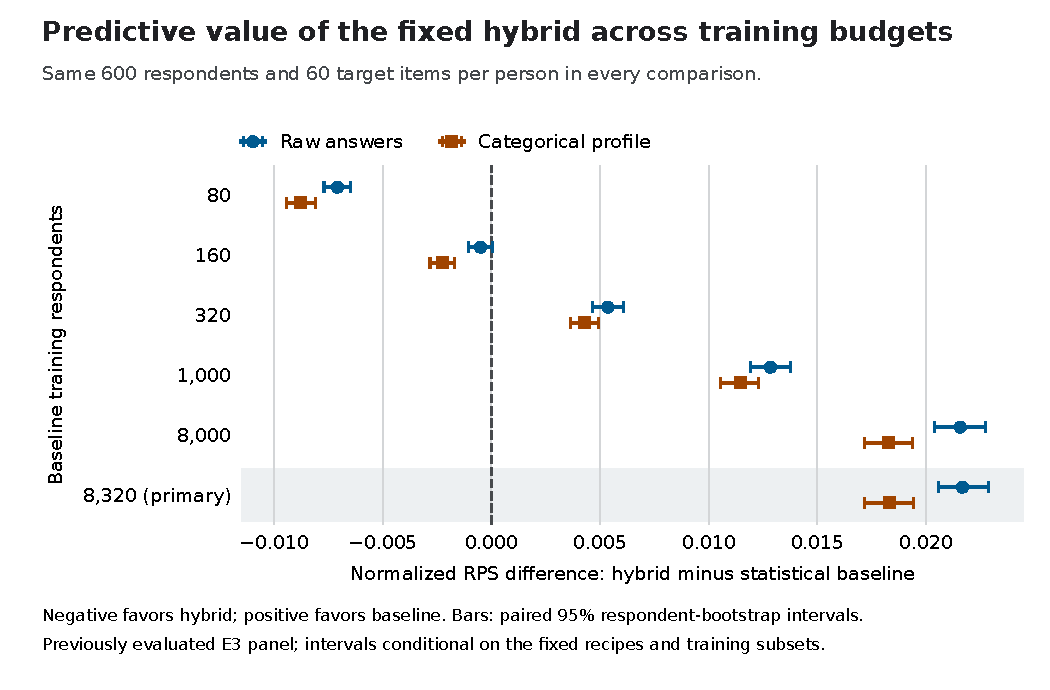
\includegraphics[width=.86\textwidth]{b1-budget.pdf}
\caption{B1 uses the same exposed E3 panel. Comparator fitting budget varies; hybrid forecasts and their larger historical supervision stay fixed. Positive hybrid-minus-comparator RPS favors the statistical predictor. Intervals are conditional on fixed fits, not uncertainty over new search runs.}
\label{fig:budget}
\end{figure*}

With 8,320 training people fixed, the mean raw-history decoder curve crosses the 60-answer hybrid's loss between ten and twenty observed answers, at an interpolated 11.44 (conditional participant interval [10.46,12.38]). Individual item orders cross at 9.17, 10.99 and 14.19. A descriptive joint participant-and-three-order bootstrap gives [9.13,13.88]; three orders do not characterize all questionnaire designs. These are decoder-relative intersections on exposed E3, not a validated shorter questionnaire or literal answer savings.

\subsection{External mixture gain is not instruction gain}
All 658 R2 TEST people have all 49 outcomes. All four standalone LLMs and four fixed-half mixtures have higher original aggregate loss than Full1400. The standalone LLMs are also worse than the history-free FIT prior (normalized risk 1.22--1.34 versus 1.000; S1). Both CAL-selected Granite mixtures improve modestly over Full1400 under the registered analysis: neutral $-0.00404$ (95\% CI $[-0.00723,-0.00096]$, Holm $p=.0360$), T0 $-0.00384$ ($[-0.00692,-0.00085]$, $p=.0486$). Both CAL-selected Qwen intervals include zero.

The direct post hoc T0-minus-neutral Granite contrast is +0.000197 ($[-0.000541,0.000957]$) under separately selected weights using the same CAL rule. At a common weight of 0.5 it is $-0.014990$ ($[-0.017155,-0.012732]$). The fixed-half contrast favors T0, but neither half-mixture beats Full1400. Standalone T0 improves Granite by 0.05703 normalized loss and worsens Qwen by 0.03066. Standalone instruction effects reverse sign across models. Shrinkage mechanically attenuates arm differences. The conditional, post hoc CAL-selected interval excludes a T0 advantage larger than 0.000541 on this scale; this is not an equivalence test or a prospective bound.

Holding decoder1200 fixed, both CAL-selected Granite mixtures also improve over their own component: neutral $-0.002886$ ($[-0.004478,-0.001282]$), T0 $-0.002689$ ($[-0.004239,-0.001123]$). Both Qwen intervals include zero. This exploratory decomposition removes comparator reselection/refitting as the sole explanation, but the mixtures still use 200 CAL outcomes for weights and require LLM forecasts. Decoder1200 minus Full1400 is $-0.001150$ ($[-0.004417,0.002007]$); that interval does not establish superiority of the smaller fit. This bridge accounts arithmetically for 28--30\% of the point gain against Full1400, without identifying the cause of the change. The bridge is favorable in the heuristic family and unfavorable in the economic family.

\begin{figure*}[t]
\centering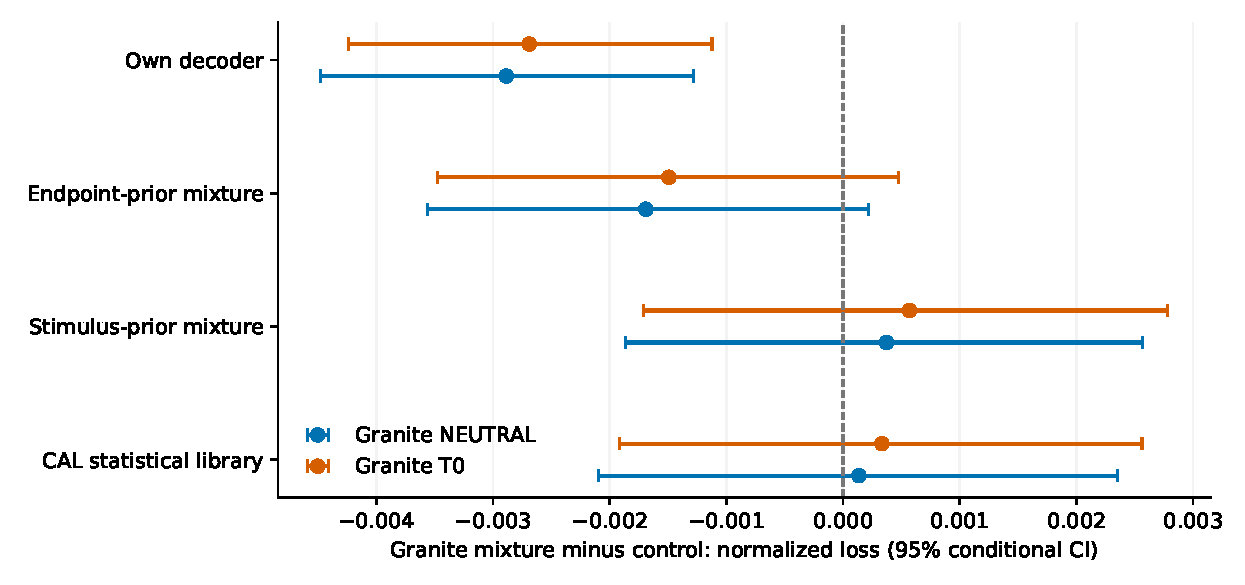
\includegraphics[width=.94\textwidth]{r2-controls.pdf}
\caption{Post-review R2 controls on saved forecasts. Fixed Granite mixtures improve their component, but intervals versus empirical-prior and statistical-library mixtures cross zero. These conditional 10,000-draw intervals do not include CAL selection variability or replace original Holm decisions. Negative favors Granite.}
\label{fig:robustness}
\end{figure*}

\subsection{Robustness to endpoint aggregation}
Under equal-endpoint weighting, both Granite mixtures still improve over their own decoder: neutral $-0.002980$ ($[-0.004438,-0.001537]$), T0 $-0.002550$ ($[-0.003924,-0.001206]$). Their original equal-family point estimates remain negative after every single-endpoint omission; the ranges are $[-0.004040,-0.002115]$ and $[-0.003596,-0.002066]$. This rules out any one endpoint as necessary for the sign of these conditional average gains, not for their statistical significance.

Against Full1400, equal-endpoint T0 gives $-0.002654$ with an interval crossing zero ($[-0.005583,0.000235]$). Neutral gives $-0.003085$ ($[-0.006059,-0.000087]$). Qwen-neutral versus its own decoder becomes slightly favorable under equal-endpoint weighting ($-0.001398$, $[-0.002819,-0.000042]$), although the original equal-family interval includes zero. We retain both aggregates and do not promote this exploratory Qwen result to registered success.

Direct Granite T0-minus-neutral remains inconclusive under equal-endpoint weighting: +0.000431 ($[-0.000338,0.001225]$). Every single-endpoint omission keeps the original equal-family point estimate positive. This provides no evidence for a favorable T0-specific CAL-mixture effect. Family contrasts and intervals are in Supplement S1b (robustness), Section 3; native absolute losses are in S1, Section 3.

Finally, adding human history to price in a separate statistical comparison increases pricing log loss by +0.00420 ($[-0.00015,0.00852]$). That interval includes zero. Strong offer prediction need not demonstrate substantial marginal value of personal history.

\subsection{Stronger controls change the positive claim}
After the first independent review, we specified additional controls on the exposed R2 outcomes before running them. We mixed decoder1200 with a FIT Laplace endpoint prior, a uniform forecast, or a FIT empirical prior conditioned on exact question text and options (including price). Each uses the same eleven weights $0,.1,\ldots,1$, endpoint CAL objective and smallest-weight tie rule. A separate statistical library chooses among all three candidates and weights on CAL (33 candidates, hence a larger search budget). No TEST outcomes choose weights or candidates. These are exploratory controls, not additions to the original Holm family.

\begin{table}[t]
\centering\small
\begin{tabular}{lrr}\toprule
Predictor & Risk & Econ. LL\\\midrule
decoder1200 & .910600 & .533033\\
Full1400 & .911749 & .532547\\
Granite neutral mixture & .907714 & .531121\\
Granite T0 mixture & .907911 & .531498\\
Endpoint-prior mixture & .909403 & .532989\\
Stimulus-prior mixture & .907341 & .530756\\
Statistical library mixture & .907577 & .531078\\\bottomrule
\end{tabular}
\caption{Absolute R2 normalized equal-family risk and economic log loss (LL). Lower is better. All mixtures select weights on CAL; control families were specified after exposure. Native ordinal and other-binary losses are in S1.}\label{tab:controls}
\end{table}

Granite neutral minus stimulus-prior mixture is +0.000373 (95\% conditional CI $[-0.001864,0.002570]$); T0 gives +0.000570 ($[-0.001706,0.002783]$). Against the CAL-selected statistical library, the corresponding differences are +0.000136 and +0.000333, both with intervals including zero. Even comparisons with endpoint-prior shrinkage include zero, whereas both Granite comparisons with the uniform mixture favor Granite. The 33-candidate library has worse TEST loss than its stimulus-prior candidate (.907577 versus .907341); CAL selection is not guaranteed to improve held-out risk. Thus these data do not establish that an LLM is needed for the small component gain. No practical-benefit margin was declared for R2; its numerical scale alone cannot establish practical value.

To probe person dependence without new inference, we also pool each Granite arm's CAL forecasts within exact stimulus cells. CAL predictions use leave-one-person-out means; TEST predictions use CAL means only. The resulting person-invariant forecast is mixed using the same grid. Personalized neutral and T0 mixtures improve over their respective proxies by $-0.002084$ ($[-0.002991,-0.001156]$) and $-0.001510$ ($[-0.002554,-0.000472]$). This conditional contrast favors personalized forecasts over the specified surrogate, but it is unadjusted, uses fixed weights, and averaging changes forecast dispersion and information; it is not a deranged-history intervention and cannot identify the causal contribution of correct personal history.

Finally, 2,000 independent CAL and TEST participant bootstrap draws reselect the original Granite weights on each CAL draw (seed 20261111). Neutral and T0 intervals versus their own fixed decoder become $[-0.004268,0.000902]$ and $[-0.003744,0.001577]$; both Full1400 intervals also include zero. The direct T0-minus-neutral interval is $[-0.000935,0.002316]$. Bootstrap mean differences versus decoder1200 are $-0.001901$ and $-0.001384$, smaller than the fixed-mixture gains; these are not bias-corrected estimates. These descriptive intervals retain fixed model fits and normalization, but expose selection sensitivity hidden by conditioning on the single selected CAL mixture. They do not replace the original fixed-pipeline inference.

\section{Discussion}
A simulator can exploit its owner's history, improve relative to neutral wording under one mixing rule, and still fail to beat a statistical alternative. Our results make these distinctions operational. For a deployable predictor, a useful evaluation should specify the instruction contrast, the available history, all human-supervision roles, the statistical comparator and calibration policy before interpreting a gain.

The reusable finding is not universal failure of personas. Granite improves its own component when the realized weights and forecasts are fixed, while Qwen and the direct transferred-instruction comparison are mixed or inconclusive. However, Granite superiority over statistical-only pooling is not established and CAL reselection widens all Granite component intervals across zero. The appropriate claim is a conditional gain of a specified pipeline, not established LLM necessity or stable population-level complementarity. The method offers a way to prevent a package gain from being attributed automatically to an instruction intervention.

Endpoint weighting expresses a target utility, not a nuisance choice to optimize after seeing outcomes. The registered aggregate remains the primary R2 target. Its sensitivity should accompany it because the nominally favorable T0-versus-Full1400 interval changes under a reasonable alternate weighting. A prospective independent panel is needed to test whether frozen instruction-specific mixtures transfer beyond these public, repeatedly analyzed outcomes.

\section{Conclusion}
We separate person matching, instruction effects and mixture gains in individual-response forecasting. Strong same-history statistical controls reverse the small-budget interpretation on IPIP. On the external survey, fixed Granite CAL mixtures improve their decoder, but stronger statistical pooling and calibration-sample uncertainty remove evidence for an LLM-specific advantage. The direct comparison also does not establish a transferred-persona advantage. Reporting the comparator budget, stimulus, calibration rule and estimand together provides a more reliable basis for deciding what a persona adds.

\section*{Limitations}
This study covers two fixed model families and two survey instruments. Public outcomes may have appeared in pretraining. E3 is disjoint from known historical panels but shares the IPIP corpus and item family; unknown lifetime exposure is unproven. B1, item-order interpolation and subsequent R2 decompositions are exploratory reuse, not independent confirmations. Post hoc control specification can also favor a statistical comparator; neither its advantage nor equivalence is independently confirmed. R2 was specified after the initial history-only CAL diagnostic. Questionnaires and hypothetical purchase choices do not validate actual behavior or interventions.

Primary intervals condition on fixed templates, decoders and calibration weights. Three historical search seeds cannot characterize general optimizer variability. Leave-one-endpoint-out sensitivity keeps the same people and task universe. The joint CAL/TEST sensitivity reselects weights but does not refit statistical models, resample their training sets, or recompute prior-loss normalization. It is not a fully nested pipeline interval. The statistical-only library does not include all alternative learned predictors, and the pooled-history surrogate cannot replace a deranged-history intervention. The attenuated T0 difference under adaptive mixing is partly expected from shrinkage; it neither proves prompt equivalence nor separates an intrinsic wording effect from forecast calibration. No equality of total supervision, pretraining or compute is established by matching the observed input or fitting-person count.

Historical serving replays exhibited Qwen drift and a separate E5 new-seed replication did not execute because its frozen pointwise compatibility gate failed. Preserving saved predictions permits scoring reproducibility but does not repair inference reproducibility. Native GigaEvo is private, so reproducing that arm requires access or a separately validated substitute. Recorded historical allocation is only a cost lower bound, omitting some failed requests, development and mutator costs.

Supplements S2--S4 preserve complete historical results and source methods; S1 records the post-review controls and uncertainty analysis. The proposed independent panel has not been recruited and contributes no empirical evidence here.

\section*{Ethical considerations and AI assistance}
We use existing questionnaire records and report aggregate results. Individual responses and forecasts remain in restricted storage; source permissions and de-identification govern release. Predictive accuracy must not be interpreted as consent to replace a person or infer sensitive attributes in deployment. New human recruitment requires separate institutional and data-protection authorization.

Codex assisted research inspection, analysis code, writing and local plotting. Claude Code provided independent manuscript critique and a generic interactive visualization template; aggregate data were bound locally. The paper figures were generated locally with matplotlib.

\bibliography{references}
\end{document}
